\chapter{Introduction}

Algorithmic trading is the process of running computer algorithms to execute orders on an electronic exchange such as NASDAQ. Speed of execution is typically paramount (and hence the alternate moniker of high-frequency trading), often requiring running the algorithms on servers directly wired to the exchange (known as co-location). Theoretically, high-frequency trading is encompassed by algorithmic trading, but not all algorithmic trading need be high-frequency; however, the two terms are often used interchangeably. 

High-frequency trading can be proprietary or non-proprietary, and varies greatly across the different types of strategies employed. For example, low-latency strategies utilize naive algorithms to profit from price discrepancies for a single stock cross-listed on multiple exchanges, while statistical arbitrage strategies use complex algorithms to profit from observed statistical patterns of a single stock on a single exchange.

Proprietary trading refers to trading for-profit with an institution's money, e.g. the livelihood of hedge funds. Cross-exchange arbitrage uses primitive algorithms and emphasizes speed: the server is co-located at one of the exchanges, algorithm latency is on the order of microseconds, and the limiting reagent is the time taken for information to travel to and from the other exchange. In the case of Chicago and New York, for example, information can make the trip in 6ms via fibreoptics that send information at half the speed of light. For this reason, agents are now paying for access to a system of ground satellites that has been set up to relay information between the two exchanges via microwaves, shaving latency down to 4ms \citep{Laughlin14}.

Non-proprietary algorithmic trading is generally aimed at transaction cost reduction, with the primary theoretical paper on the subject being \citet{Bertsimas98} and \citet{Almgren01}. When an institutional investor wishes to buy or sell a large quantity of shares, the aim of the trader is to obtain the best possible price compared with some benchmark (often taken to be the midprice at the time of initiating the strategy). Here the definition of `large' is determined relative to the liquidity of the stock - either in comparison to the average size of trades for the given stock, or to the available quantity to be bought/sold at the best listed price. The goal of the algorithmic trading is then to split up the large order into smaller pieces and execute them on an algorithmically-determined schedule, balancing the total time for execution with the volatility of the price the trader will receive. 

In statistical arbitrage, the aim is to exploit predictable statistical patterns in the available data provided by the exchange, e.g. predicting stock price movements from prices observed thus far. This method too requires co-location, and operates on the scale of milliseconds. It is this type of high-frequency trading that I will explore in this dissertation. 

As part of the Dodd-Frank Act of 2010, the Volcker Rule has banned US banks from making certain speculative investments, and in so doing effectively curbed their proprietary trading activity. Nevertheless, as they are still required to provide liquidity to markets via market-making, banks utilize algorithmic trading to determine the bid/ask bands they will send to exchanges. Thus it remains feasible for banks to simply shift the bands they send in order to comply with market-making requirements and simultaneously execute a given strategy.

\section{Limit Order Book Dynamics}

A \emph{limit order} is an instruction submitted by an agent to buy or sell up to a specified quantity or volume of a financial instrument, and at a specified price. A \emph{limit order book (LOB)} is the accumulated list of such orders sent to a given exchange, where each order is accompanied by a timestamp and an anonymous unique key for identifying the agent. The exchange runs a trade matching engine that utilizes the LOB to pair buy and sell requests that concur on price, even if only partially on volume. Orders remain in effect until they are modified, canceled, or fully filled \citep{Kyle1989}.

The unfilled or partially filled orders accumulate in the limit order book and provide liquidity to the market. At any given time, the structure of the LOB can be visualized as in \autoref{fig:LOB}. As new limit orders arrive, they are compared with existing opposing orders in the book in search of a match - and if so, existing orders are \emph{filled} or \emph{lifted} according to a first-in-first-out priority queue for each price level. \emph{Market orders} extend the idea of limit orders by specifying only the volume, and accept the best possible price currently available in the LOB; whereas limit orders are free to post, modify, and cancel (as an incentive for providing liquidity), market orders are charged a fee.

\begin{figure}
  \tikzsetnextfilename{LOB}
  %\documentclass{article}
%\usepackage{pgfplots}
%\usetikzlibrary{backgrounds}
%\begin{document}
% Limit Order Book structure and mechanics by Anton, inspired by Ash Booth
\pgfdeclarepatternformonly[\LineSpace]{myhatch}{\pgfqpoint{-1pt}{-1pt}}{\pgfqpoint{\LineSpace}{\LineSpace}}{\pgfqpoint{\LineSpace}{\LineSpace}}%
{
    \pgfsetlinewidth{1pt}
    \pgfpathmoveto{\pgfqpoint{0pt}{\LineSpace}}
    \pgfpathlineto{\pgfqpoint{\LineSpace + 0.1pt}{-0.1pt}}
    \pgfusepath{stroke}
}

\newdimen\LineSpace
\tikzset{
    line space/.code={\LineSpace=#1},
    line space=5pt
}

\colorlet{buyLOcolor}{black!25}%
\colorlet{sellLOcolor}{black!90}%
\begin{center}%
\makebox[0pt]{%
\begin{tikzpicture}[
	/pgf/number format/fixed,
	/pgf/number format/fixed zerofill,	
	/pgf/number format/precision=2,
	buyLOone/.style ={rectangle,draw=black, fill=buyLOcolor,thick,outer sep = 0.05cm,minimum size=0.9cm,anchor=south,rounded corners=0.2cm},
	buyLOonematch/.style ={rectangle,draw=black,thick,outer sep=0.05cm,minimum size=0.9cm,anchor=south,rounded corners=0.2cm,preaction={fill=buyLOcolor},pattern=myhatch},
	buyLOtwo/.style ={rectangle,draw=black, fill=buyLOcolor,thick,outer sep = 0.05cm,minimum height =1.9cm ,minimum width=0.9cm,anchor=south,rounded corners=0.2cm},
	buyLOthree/.style ={rectangle,draw=black, fill=buyLOcolor,thick,outer sep = 0.05cm,minimum height=2.9cm,minimum width=0.9cm,anchor=south,rounded corners=0.2cm},
	sellLOone/.style ={rectangle,draw=black, fill=sellLOcolor,thick,outer sep = 0.05cm,minimum size=0.9cm,anchor=south,rounded corners=0.2cm},
	sellLOtwo/.style ={rectangle,draw=black, fill=sellLOcolor,thick,outer sep = 0.05cm,minimum height=1.9cm ,minimum width=0.9cm,anchor=south,rounded corners=0.2cm},
	sellLOthree/.style ={rectangle,draw=black, fill=sellLOcolor,thick,outer sep = 0.05cm,minimum height=2.9cm,minimum width=0.9cm,anchor=south,rounded corners=0.2cm}]
    \draw [>=latex,->] (-0.55,-0.05) -- (12,-0.05) node[draw=none,fill=none,midway,shift=(down:1),font=\Large] {Price};
    \draw [>=latex,->] (-0.55,-0.05) -- (-0.55,9) node[draw=none,fill=none,midway,rotate=90,shift=(up:0.75),font=\Large] {Volume};
    
    \foreach \x [evaluate=\x as \price using \x/100 + 28.90]  in {0,...,11} \draw (\x ,-0.05) -- (\x ,-0.1) node[anchor=north] {$\scriptstyle\pgfmathprintnumber{\price}$};

%%% LOB
	\node[buyLOone]			at (0,0) {};
	\node[buyLOone]			at (0,1) {};
	\node[buyLOtwo]			at (1,0) {};
	\node[buyLOone]			at (1,2) {};
	\node[buyLOthree]		at (2,0) {};
	\node[buyLOtwo]			at (3,0) {};
	\node[buyLOtwo]			at (3,2) {};
	\node[buyLOtwo]			at (3,4) {};
	\node[buyLOonematch]	at (4,0) {};
	\node[buyLOonematch]	at (4,1) {};
	\node[buyLOtwo] 		at (4,2) {};
	\node[buyLOone] 		at (4,4) {};
	
	\node[sellLOone]			at (7,0) {};
	\node[sellLOone]			at (7,1) {};
	\node[sellLOone]			at (7,2) {};
	\node[sellLOtwo]			at (8,0) {};
	\node[sellLOtwo]			at (10,0) {};
	\node[sellLOthree]		at (11,0) {};
	\node[sellLOthree]		at (11,3) {};

%%% BID ASK SPREAD
	\draw [<->] (5,1.5)  -- (6,1.5) node[midway, anchor=north, text width=2cm, align=center, thick] {Bid-Ask \\ Spread};

%%% MARKET ORDER		
	\node[sellLOtwo]			at (4,7) {};
	\draw[->, ultra thick] (4,7) -- (4,0.5);
	\node at (3.5,9) [anchor=north east, text width=3cm, align=right, font=\tiny] {A market order to sell two shares arrives, and matches with the first two limit orders in the queue at the best price.};
	
%%% LIMIT ORDER
	\node[sellLOone]			at (7,5) {};
	\draw[->, ultra thick] (7,5) -- (7,3);
	\node at (7.5,6) [anchor=north west, text width=2cm, align=left, font=\tiny] {A limit order to sell one share at 28.97 arrives, and is added to the back of the queue.};	
	
%%% LEGEND
	\node[buyLOone]			at (8,8) {};
	\node[sellLOone]			at (8,7) {};
	\node at (8.5,8.5) [anchor=west, align=left] {Bid (buy) LO};
	\node at (8.5,7.5) [anchor=west, align=left] {Ask (sell) LO};
\end{tikzpicture}
}
\end{center}
%\end{document}

%  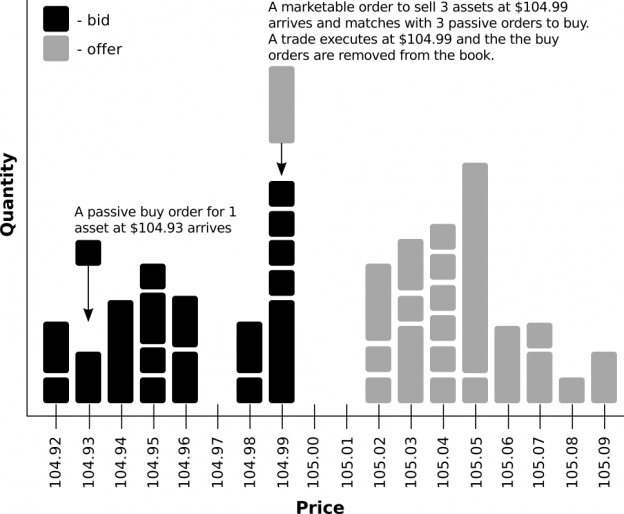
\includegraphics[width=0.9\textwidth]{Figs/LOBAshBooth.png}
\caption{Structure and mechanics of the limit order book, adapted from \citet{Booth15}. Each block represents an order, of varying volumes, submitted by an agent.}
\label{fig:LOB}
\end{figure}

In the literature, LOBs are generally modelled in one of two ways: either by an economics-based approach, or a physics-based approach \citep{Summary2013}. The economics based approaches are trader-centric, assume perfect rationality, view order flow as static, and seek to understand trader strategies, in particular through game-style theories. By contrast, the physics approach, with which we are more concerned here, assumes zero-intelligence, provides conceptual toy models of the evolution of the book, and is concerned with the search for statistical regularity. The dynamics of the book, namely order arrivals and cancellations, are governed by stochastic processes of varying complexity, from particles on a 1-D price lattice \citep{Bak97} to independent Poisson processes governing the arrival, modification, and cancellation of orders \citep{Cont10}. See \citet{Summary2013} for an excellent literature survey on LOB modelling.

In this thesis, I will be concerned primarily with limit order book order imbalance. \emph{Imbalance} is a ratio of limit order volumes between the bid and ask side, and in this work is calculated as 
\begin{equation}\label{eq:LOBImbalance}
I(t) = \dfrac{V_{bid}(t) - V_{ask}(t)}{V_{bid}(t) + V_{ask}(t)} \in [-1,1]
\end{equation}
where both $V_{bid}$ and $V_{ask}$ are computed as the weighted average volumes at the best three prices, with exponentially decreasing weights.

\section{ITCH Data Set}
\fxnote{write ITCH data set section.}